\documentclass{article}
    % General document formatting
    \usepackage[margin=0.7in]{geometry}
    \usepackage[parfill]{parskip}
    \usepackage[T5]{fontenc}
    \usepackage[utf8]{inputenc}
    \usepackage{amsmath}
    \usepackage{tikz}
    \usepackage{fancyhdr}

\pagestyle{fancy}
\fancyhf{}
\rhead{Edgar Jacob Rivera Rios - A01184125}

\begin{document}
a) Show that for any x, $x \in A + B$ iff x is an element of exactly one of A, B
\begin{equation*}
    x \in A + B \implies (x \in A \cap x \notin B) \cup (x \in B \cap x \notin A)
\end{equation*}
b) Draw a Venn diagram for the operation\\
\begin{center}
    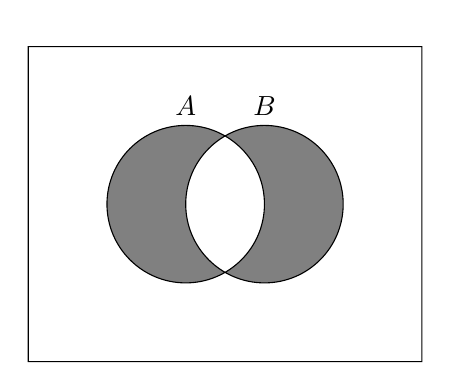
\begin{tikzpicture}[fill=gray]
        % left hand
        \scope
        \clip (-2,-2) rectangle (2,2)
            (1,0) circle (1);
        \fill (0,0) circle (1);
        \endscope
        % right hand
        \scope
        \clip (-2,-2) rectangle (2,2)
            (0,0) circle (1);
        \fill (1,0) circle (1);
        \endscope
        % outline
        \draw (0,0) circle (1) (0,1)  node [text=black,above] {$A$}
            (1,0) circle (1) (1,1)  node [text=black,above] {$B$}
            (-2,-2) rectangle (3,2) node [text=black,above] {};
    \end{tikzpicture}
\end{center}
(c) Show that $A+B \subseteq A \cup B$ \\
\begin{equation*}
    x \in A+B \implies (x \in A \cap x \notin B) \cup (x \in B \cap x \notin A)
\end{equation*}
\begin{align*}
    x \in A \cup B &\implies x \in A \cup x \in B\\
                   &\implies A = B
\end{align*}
(d) Show that $A+B$ is disjoint from $A \cap B$.\\
(e) Show that $A+B = (A \cup B)|(A \cap B)$.\\
(f) For each of the following properties of $\cup$ , check out whether or not it also holds for +, giving a proof or a counter example as appropriate: (i) commutativity, (ii) associativity, (iii) distribution of over +, (iv) distribution of + over $\cap$.\\
(g) Express $-(A+B)$ using union, intersection and complement.\\
\begin{align*}
    -(A+B) &\implies -((A|B) \cup (B|A))\\
           &\implies (A \cap B') \cup (B \cap A')'\\
           &\implies (A \cap B) \cup (A' \cap B')\\
\end{align*}
(h) We have seen that each of intersection, union and difference corresponds to a truth-functional logical connective. To what connective mentioned in this lecture does symmetric difference correspond? Draw its truth table.
\begin{table}[h!]
    \label{tab:table1}
    \centering
    \begin{tabular}{c|c|c}
        \textbf{A} & \textbf{B} & \textbf{$A+B$}\\
        \hline
        1 & 1 & 0\\
        \hline
        1 & 0 & 1\\
        \hline
        0 & 1 & 1\\
        \hline
        0 & 0 & 0\\
    \end{tabular}
\end{table}
\end{document}